% Options for packages loaded elsewhere
\PassOptionsToPackage{unicode}{hyperref}
\PassOptionsToPackage{hyphens}{url}
\PassOptionsToPackage{dvipsnames,svgnames,x11names}{xcolor}
%
\documentclass[
]{scrartcl}

\usepackage{amsmath,amssymb}
\usepackage{iftex}
\ifPDFTeX
  \usepackage[T1]{fontenc}
  \usepackage[utf8]{inputenc}
  \usepackage{textcomp} % provide euro and other symbols
\else % if luatex or xetex
  \usepackage{unicode-math}
  \defaultfontfeatures{Scale=MatchLowercase}
  \defaultfontfeatures[\rmfamily]{Ligatures=TeX,Scale=1}
\fi
\usepackage{lmodern}
\ifPDFTeX\else  
    % xetex/luatex font selection
\fi
% Use upquote if available, for straight quotes in verbatim environments
\IfFileExists{upquote.sty}{\usepackage{upquote}}{}
\IfFileExists{microtype.sty}{% use microtype if available
  \usepackage[]{microtype}
  \UseMicrotypeSet[protrusion]{basicmath} % disable protrusion for tt fonts
}{}
\makeatletter
\@ifundefined{KOMAClassName}{% if non-KOMA class
  \IfFileExists{parskip.sty}{%
    \usepackage{parskip}
  }{% else
    \setlength{\parindent}{0pt}
    \setlength{\parskip}{6pt plus 2pt minus 1pt}}
}{% if KOMA class
  \KOMAoptions{parskip=half}}
\makeatother
\usepackage{xcolor}
\setlength{\emergencystretch}{3em} % prevent overfull lines
\setcounter{secnumdepth}{3}
% Make \paragraph and \subparagraph free-standing
\ifx\paragraph\undefined\else
  \let\oldparagraph\paragraph
  \renewcommand{\paragraph}[1]{\oldparagraph{#1}\mbox{}}
\fi
\ifx\subparagraph\undefined\else
  \let\oldsubparagraph\subparagraph
  \renewcommand{\subparagraph}[1]{\oldsubparagraph{#1}\mbox{}}
\fi

\providecommand{\tightlist}{%
  \setlength{\itemsep}{0pt}\setlength{\parskip}{0pt}}\usepackage{longtable,booktabs,array}
\usepackage{calc} % for calculating minipage widths
% Correct order of tables after \paragraph or \subparagraph
\usepackage{etoolbox}
\makeatletter
\patchcmd\longtable{\par}{\if@noskipsec\mbox{}\fi\par}{}{}
\makeatother
% Allow footnotes in longtable head/foot
\IfFileExists{footnotehyper.sty}{\usepackage{footnotehyper}}{\usepackage{footnote}}
\makesavenoteenv{longtable}
\usepackage{graphicx}
\makeatletter
\def\maxwidth{\ifdim\Gin@nat@width>\linewidth\linewidth\else\Gin@nat@width\fi}
\def\maxheight{\ifdim\Gin@nat@height>\textheight\textheight\else\Gin@nat@height\fi}
\makeatother
% Scale images if necessary, so that they will not overflow the page
% margins by default, and it is still possible to overwrite the defaults
% using explicit options in \includegraphics[width, height, ...]{}
\setkeys{Gin}{width=\maxwidth,height=\maxheight,keepaspectratio}
% Set default figure placement to htbp
\makeatletter
\def\fps@figure{htbp}
\makeatother
\newlength{\cslhangindent}
\setlength{\cslhangindent}{1.5em}
\newlength{\csllabelwidth}
\setlength{\csllabelwidth}{3em}
\newlength{\cslentryspacingunit} % times entry-spacing
\setlength{\cslentryspacingunit}{\parskip}
\newenvironment{CSLReferences}[2] % #1 hanging-ident, #2 entry spacing
 {% don't indent paragraphs
  \setlength{\parindent}{0pt}
  % turn on hanging indent if param 1 is 1
  \ifodd #1
  \let\oldpar\par
  \def\par{\hangindent=\cslhangindent\oldpar}
  \fi
  % set entry spacing
  \setlength{\parskip}{#2\cslentryspacingunit}
 }%
 {}
\usepackage{calc}
\newcommand{\CSLBlock}[1]{#1\hfill\break}
\newcommand{\CSLLeftMargin}[1]{\parbox[t]{\csllabelwidth}{#1}}
\newcommand{\CSLRightInline}[1]{\parbox[t]{\linewidth - \csllabelwidth}{#1}\break}
\newcommand{\CSLIndent}[1]{\hspace{\cslhangindent}#1}

\usepackage{scrlayer-scrpage}
\usepackage{lastpage}
\lohead{ATLS vs Standard Care Trial SAP}
\rohead{ClinicalTrials.gov ID NCT06321419}
\cfoot{\thepage\ of \pageref{LastPage} }
\makeatletter
\makeatother
\makeatletter
\makeatother
\makeatletter
\@ifpackageloaded{caption}{}{\usepackage{caption}}
\AtBeginDocument{%
\ifdefined\contentsname
  \renewcommand*\contentsname{Table of contents}
\else
  \newcommand\contentsname{Table of contents}
\fi
\ifdefined\listfigurename
  \renewcommand*\listfigurename{List of Figures}
\else
  \newcommand\listfigurename{List of Figures}
\fi
\ifdefined\listtablename
  \renewcommand*\listtablename{List of Tables}
\else
  \newcommand\listtablename{List of Tables}
\fi
\ifdefined\figurename
  \renewcommand*\figurename{Figure}
\else
  \newcommand\figurename{Figure}
\fi
\ifdefined\tablename
  \renewcommand*\tablename{Table}
\else
  \newcommand\tablename{Table}
\fi
}
\@ifpackageloaded{float}{}{\usepackage{float}}
\floatstyle{ruled}
\@ifundefined{c@chapter}{\newfloat{codelisting}{h}{lop}}{\newfloat{codelisting}{h}{lop}[chapter]}
\floatname{codelisting}{Listing}
\newcommand*\listoflistings{\listof{codelisting}{List of Listings}}
\makeatother
\makeatletter
\@ifpackageloaded{caption}{}{\usepackage{caption}}
\@ifpackageloaded{subcaption}{}{\usepackage{subcaption}}
\makeatother
\makeatletter
\@ifpackageloaded{tcolorbox}{}{\usepackage[skins,breakable]{tcolorbox}}
\makeatother
\makeatletter
\@ifundefined{shadecolor}{\definecolor{shadecolor}{rgb}{.97, .97, .97}}
\makeatother
\makeatletter
\makeatother
\makeatletter
\makeatother

\usepackage{hyphenat}
\usepackage{ifthen}
\usepackage{calc}
\usepackage{calculator}



\usepackage{graphicx}
\usepackage{geometry}
\usepackage{afterpage}
\usepackage{tikz}
\usetikzlibrary{calc}
\usetikzlibrary{fadings}
\usepackage[pagecolor=none]{pagecolor}


% Set the titlepage font families







% Set the coverpage font families

\ifLuaTeX
  \usepackage{selnolig}  % disable illegal ligatures
\fi
\IfFileExists{bookmark.sty}{\usepackage{bookmark}}{\usepackage{hyperref}}
\IfFileExists{xurl.sty}{\usepackage{xurl}}{} % add URL line breaks if available
\urlstyle{same} % disable monospaced font for URLs
\hypersetup{
  pdftitle={Statistical Analysis Plan},
  pdfauthor={Version 0.3.0, 2024-09-18},
  colorlinks=true,
  linkcolor={blue},
  filecolor={Maroon},
  citecolor={Blue},
  urlcolor={Blue},
  pdfcreator={LaTeX via pandoc}}

\title{Statistical Analysis Plan}
\usepackage{etoolbox}
\makeatletter
\providecommand{\subtitle}[1]{% add subtitle to \maketitle
  \apptocmd{\@title}{\par {\large #1 \par}}{}{}
}
\makeatother
\subtitle{ADVANCE TRAUMA\\
\strut \\
Effects of Advanced Trauma Life Support\textsuperscript{®} Training
Compared to Standard Care on Adult Trauma Patient Outcomes: A Cluster
Randomised Trial}
\author{Version 0.3.0, 2024-09-18}
\date{}

\begin{document}
%%%%% begin titlepage extension code


\begin{titlepage}

%%% TITLE PAGE START

% Set up alignment commands
%Page
\newcommand{\titlepagepagealign}{
\ifthenelse{\equal{center}{right}}{\raggedleft}{}
\ifthenelse{\equal{center}{center}}{\centering}{}
\ifthenelse{\equal{center}{left}}{\raggedright}{}
}


\newcommand{\titleandsubtitle}{
% Title and subtitle
{\fontsize{15}{18.0}\selectfont
{\uppercase{\nohyphens{Statistical Analysis Plan}}}\par
}%

\vspace{\betweentitlesubtitle}
{
\fontsize{20}{24.0}\selectfont
{\bfseries{\nohyphens{ADVANCE TRAUMA\\
\strut \\
Effects of Advanced Trauma Life Support\textsuperscript{®} Training
Compared to Standard Care on Adult Trauma Patient Outcomes: A Cluster
Randomised Trial}}}\par
}}
\newcommand{\titlepagetitleblock}{
\rule{\textwidth}{0.4pt} % Thin horizontal rule
\vspace{0.025\textheight} % Whitespace between the top rules and title

\titleandsubtitle

\vspace{0.025\textheight} 
\rule{0.3\textwidth}{0.4pt} % Short horizontal rule under the title
}
\newcommand{\authorstyle}[1]{{\Large{#1}}}

\newcommand{\affiliationstyle}[1]{{\large{#1}}}

\newcommand{\titlepageauthorblock}{
{\authorstyle{\nohyphens{Version 0.3.0, 2024-09-18}\\}}
}

\newcommand{\titlepageaffiliationblock}{
\hangindent=1em
\hangafter=1
{\affiliationstyle{


\vspace{1\baselineskip} 
}}
}
\newcommand{\headerstyled}{%
{}
}
\newcommand{\footerstyled}{%
{\large{\textsc{}}}
}
\newcommand{\datestyled}{%
{}
}


\newcommand{\titlepageheaderblock}{\headerstyled}

\newcommand{\titlepagefooterblock}{
\footerstyled
}

\newcommand{\titlepagedateblock}{
\datestyled
}

%set up blocks so user can specify order
\newcommand{\titleblock}{\newlength{\betweentitlesubtitle}
\setlength{\betweentitlesubtitle}{\baselineskip}
{

{\titlepagetitleblock}
}

\vspace{0.1\textheight}
}

\newcommand{\authorblock}{{\titlepageauthorblock}

\vspace{2\baselineskip}
}

\newcommand{\affiliationblock}{{\titlepageaffiliationblock}

\vspace{1pt}
}

\newcommand{\logoblock}{}

\newcommand{\footerblock}{}

\newcommand{\dateblock}{}

\newcommand{\headerblock}{}

\thispagestyle{empty} % no page numbers on titlepages


\newlength{\minipagewidth}
\setlength{\minipagewidth}{\textwidth}
\raggedright % single minipage
% [position of box][box height][inner position]{width}
% [s] means stretch out vertically; assuming there is a vfill
\begin{minipage}[b][\textheight][s]{\minipagewidth}
\titlepagepagealign
\titleblock

\authorblock

\vfill

\logoblock

\footerblock
\par

\end{minipage}\ifthenelse{\equal{}{right} \OR \equal{}{leftright} }{
\hspace{\B}
\vrulecode}{}
\clearpage
%%% TITLE PAGE END
\end{titlepage}
\setcounter{page}{1}

%%%%% end titlepage extension code
\ifdefined\Shaded\renewenvironment{Shaded}{\begin{tcolorbox}[breakable, boxrule=0pt, frame hidden, interior hidden, borderline west={3pt}{0pt}{shadecolor}, enhanced, sharp corners]}{\end{tcolorbox}}\fi

\renewcommand*\contentsname{Table of contents}
{
\hypersetup{linkcolor=}
\setcounter{tocdepth}{3}
\tableofcontents
}
\newpage{}

\hypertarget{administrative-information}{%
\section{Administrative information}\label{administrative-information}}

\hypertarget{study-identifiers}{%
\subsection{Study identifiers}\label{study-identifiers}}

\begin{itemize}
\tightlist
\item
  Protocol version 1.2.0 dated 2024-08-26
\item
  ClinicalTrials.gov ID NCT06321419
\item
  Clinical Trial Registry - India
\end{itemize}

\hypertarget{changelog}{%
\subsection{Changelog}\label{changelog}}

Once version 1.0.0 is finalised, this section will be updated with a
changelog.

\hypertarget{contributors}{%
\subsection{Contributors}\label{contributors}}

\newpage{}

\hypertarget{trial-synopsis}{%
\section{Trial synopsis}\label{trial-synopsis}}

\textbf{Title} Effects of Advanced Trauma Life
Support\textsuperscript{®} Training Compared to Standard Care on Adult
Trauma Patient Outcomes: A Cluster Randomised Trial

\textbf{Rationale} Trauma is a massive global health issue. Many
training programmes have been developed to help physicians in the
initial management of trauma patients. Among these programmes, Advanced
Trauma Life Support\textsuperscript{®} (ATLS\textsuperscript{®}) is the
most popular, having trained over one million physicians worldwide.
Despite its widespread use, there are no controlled trials showing that
ATLS\textsuperscript{®} improves patient outcomes. Multiple systematic
reviews emphasise the need for such trials.

\textbf{Aim} To compare the effects of ATLS\textsuperscript{®} training
with standard care on outcomes in adult trauma patients.

\textbf{Primary Outcome} In-hospital mortality within 30 days of arrival
at the emergency department.

\textbf{Trial Design} Batched stepped-wedge cluster randomised trial in
India.

\textbf{Trial Population} Adult trauma patients presenting to the
emergency department of a participating hospital.

\textbf{Sample Size} 30 clusters and 4320 patients.

\textbf{Eligibility Criteria}

\emph{Hospitals} are secondary or tertiary hospitals in India that admit
or refer/transfer for admission at least 400 patients with trauma per
year.

\emph{Clusters} are one or more units of physicians providing initial
trauma care in the emergency department of tertiary hospitals in India.

\emph{Patients participants} are adult trauma patients who presents to
the emergency department of participating hospitals and are admitted or
transferred for admission.

\textbf{Intervention} The intervention will be ATLS\textsuperscript{®}
training, a proprietary 2.5 day course teaching a standardised approach
to trauma patient care using the concepts of a primary and secondary
survey. Physicians will be trained in an accredited
ATLS\textsuperscript{®} training facility in India.

\textbf{Ethical Considerations} We will use an opt-out consent approach
for collection of routinely recorded data. We will obtain informed
consent for collection of non-routinely recorded data, such as quality
of life and disability outcomes. Patients who are unconscious or lack a
legally authorized representative will be included under a waiver of
informed consent. Note that consent here refers to consent to data
collection.

\textbf{Trial Period} October 1, 2024, to September 30, 2029

\newpage{}

\hypertarget{special-considerations}{%
\section{Special considerations}\label{special-considerations}}

\hypertarget{funding}{%
\subsection{Funding}\label{funding}}

This trial is not yet fully funded. The Trial Management Group has
decided to proceed with the trial with the expectation that additional
funding will be secured. The Trial Steering Committee will be informed
of the funding status at each meeting. If funding is not secured, the
trial will be stopped. This will likely result in an underpowered trial.
The justification for this decision is that the intervention is
considered standard of care in many countries and the data collection is
considered minimal risk. There is therefore a very small risk of harm to
patient participants, but a potential direct benefit to those patient
participants who receive the intervention. The benefit-risk ratio is
therefore considered to be favourable, even in the case of an
underpowered trial.

\hypertarget{potential-amendments}{%
\subsection{Potential amendments}\label{potential-amendments}}

There are ongoing discussions about re-framing the trial as a hybrid
effectiveness-implementation trial and include a cost-effectiveness
analysis. This would involve adding additional data collection to assess
the implementation and costs of the intervention. This would involve
additional funding and amended ethical approvals.

\newpage{}

\hypertarget{statistical-analysis}{%
\section{Statistical analysis}\label{statistical-analysis}}

\hypertarget{aim-and-objectives}{%
\section{Aim and objectives}\label{aim-and-objectives}}

\hypertarget{aim}{%
\subsection{Aim}\label{aim}}

To compare the effects of ATLS\textsuperscript{®} training with standard
care on outcomes in adult trauma patients.

\hypertarget{objectives}{%
\subsection{Objectives}\label{objectives}}

\begin{itemize}
\tightlist
\item
  To estimate the effects of ATLS\textsuperscript{®} training on 30-day
  in-hospital mortality compared to standard care.
\item
  To assess the robustness of the main analysis results to different
  model specifications through sensitivity analyses.
\item
  To estimate the effects of ATLS\textsuperscript{®} training on
  secondary outcomes compared to standard care.
\item
  To explore the effects of ATLS\textsuperscript{®} training on
  subgroups of patients compared to standard care.
\end{itemize}

\hypertarget{design}{%
\subsection{Design}\label{design}}

This is a batched stepped-wedge cluster randomised trial, including a
total of 30 (see\textsuperscript{\textbf{trial-design?}}). The trial
will be composed of 6 batches of identical 12-period 5-sequence design,
with one cluster being assigned to each sequence of each
batch\textsuperscript{1}. Each period is one month, and each cluster
will be in the trial for a total of 13 months. The intervention will be
implemented during a one-month transition period, which will be excluded
from the analysis. There will be an overlap of 6 months between
successive batches.

\begin{figure}

{\centering 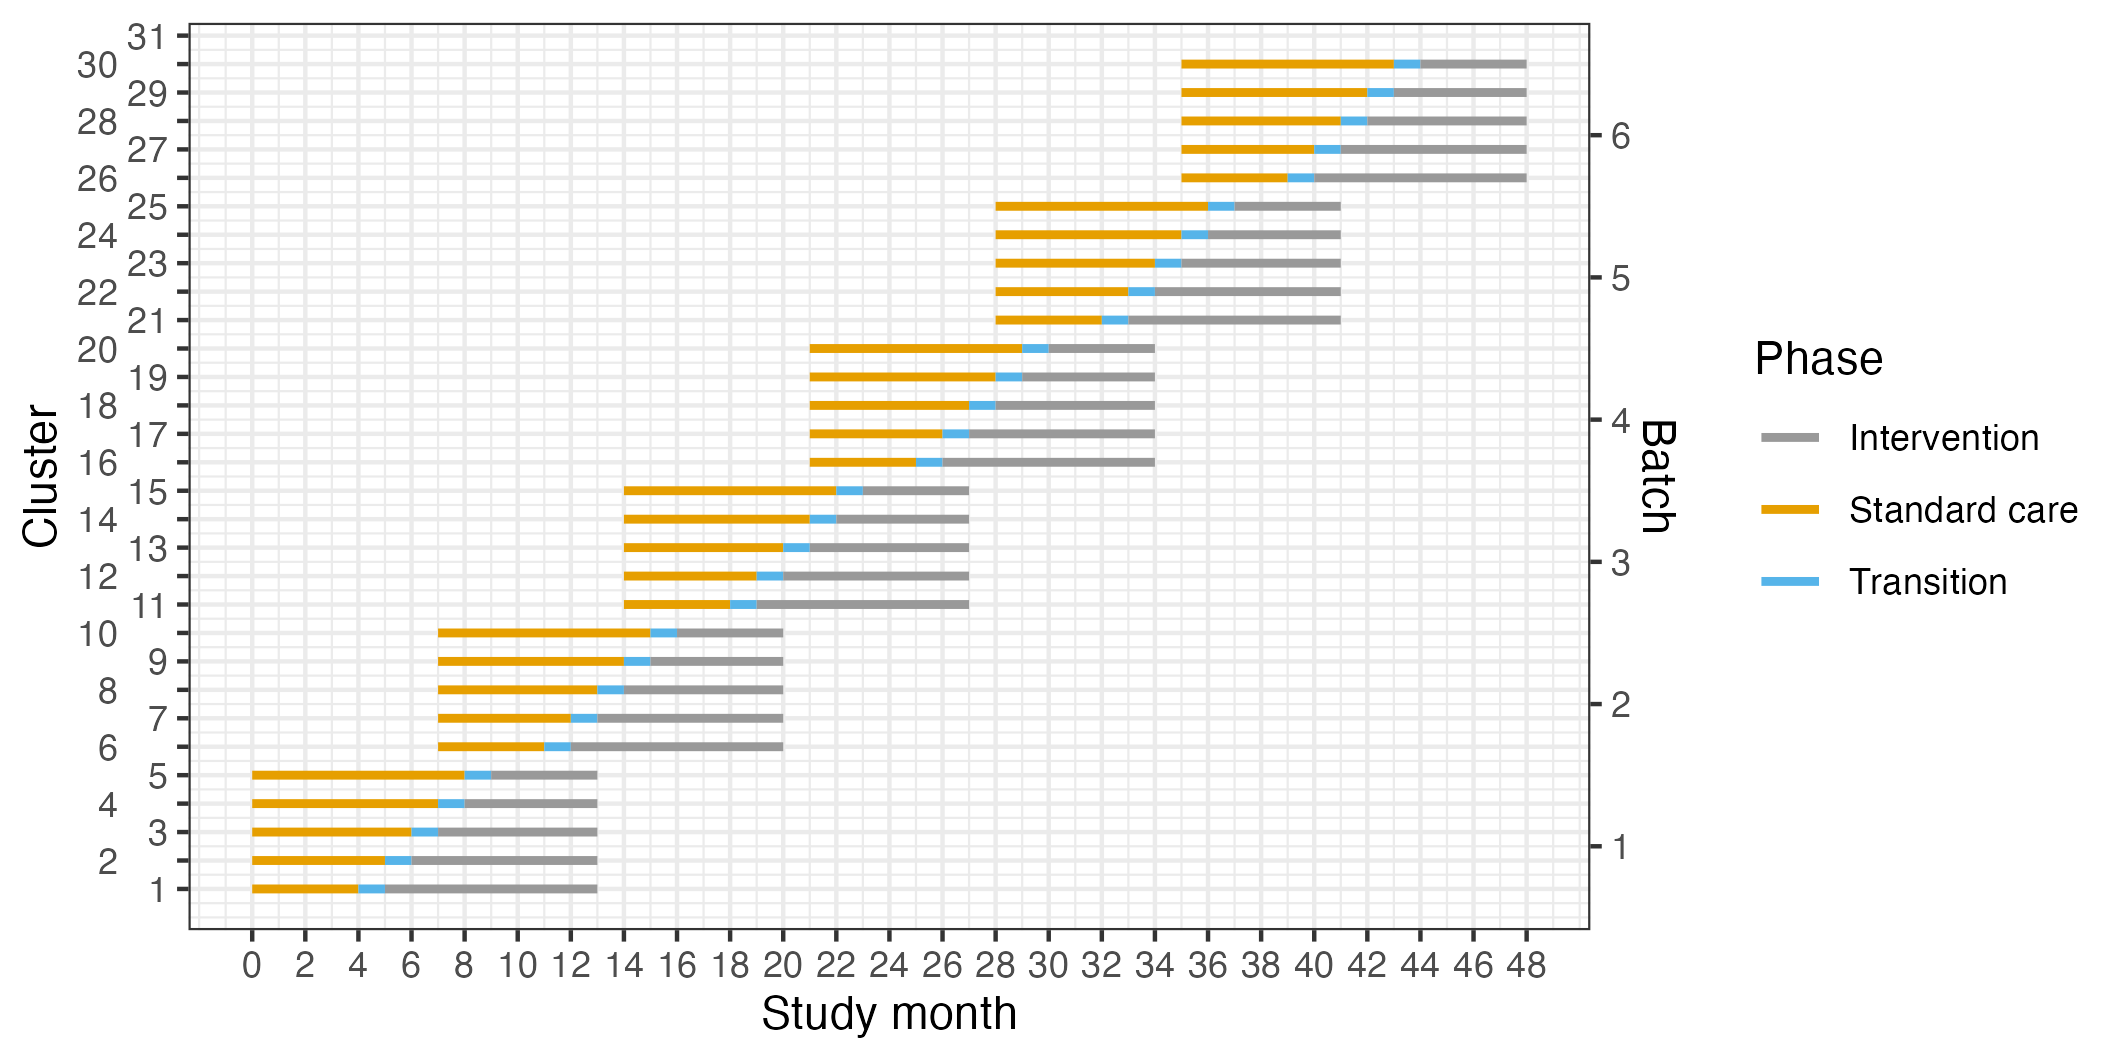
\includegraphics{trial-design-figure-30-clusters-5-sequences-6-batches-6-batches-overlap-4-min-standard-care-4-min-intervention-1-transition-months-0-transition-overlap.png}

}

\caption{\label{fig-trial-design}Trial design. Lines represent the
duration of patient enrolment across clusters and phases. Clusters will
be sequentially allocated to a batch based on when they enter the study.
Within each batch clusters will then be randomised to an intervention
implementation sequence.}

\end{figure}

\hypertarget{randomisation-of-clusters}{%
\subsection{Randomisation of clusters}\label{randomisation-of-clusters}}

We will assign clusters to batches as they are found to be eligible and
receive ethical approval. Batches will include clusters from hospitals
in different regions to optimize trial logistics. We will randomise the
clusters alloted to each batch to the different intervention
implementation sequences within that batch\footnote{\textbf{Question:}
  Karla and James, can you please provide more details on how the
  randomisation will be done?}. We will balance the randomisation within
each batch on cluster size, defined as monthly volume of eligible
patient participants, using covariate constrained randomisation. The
cluster sizes are expected to vary between 12 and 20 patients per month,
based on our previous experiences. We will conceal the randomisation
order for as long as it is logistically possible, considering that
arrangements for sending physicians to ATLS\textsuperscript{®} training
need to be made in advance.

\hypertarget{outcomes}{%
\subsection{Outcomes}\label{outcomes}}

\hypertarget{primary-outcome}{%
\subsubsection{Primary outcome}\label{primary-outcome}}

The primary outcome will be in-hospital mortality within 30 days of
arrival at the emergency department. Clinical research coordinators will
extract information on death from patient hospital records. If the
patient has been transferred to another hospital, the clinical research
coordinators will collect data on this outcome by calling the patient or
a patient representative, or by contacting the hospital to which the
patient was transferred. Data on this outcome will be collected
continuously during the trial.

\hypertarget{secondary-outcomes}{%
\subsubsection{Secondary outcomes}\label{secondary-outcomes}}

\begin{itemize}
\tightlist
\item
  All cause mortality within 24 hours, 30 days and three months of
  arrival at the emergency department. Data on this outcome will be
  collected in the same way as for the primary outcome.
\item
  Quality of life within seven days of discharge, and at 30 days and
  three months of arrival at the emergency department, measured by the
  official and validated translations of the EQ5D3L. Data on this
  outcome will be collected in person if the patient is still in
  hospital, or by phone if the patient has been discharged. We will
  collect this data from a stratified random sample (site and period) of
  patient participants. The sampling will be designed so that is
  maximises statistical efficiency.
\item
  Disability within seven days of discharge, and at 30 days and three
  months of arrival at the emergency department, assessed using the WHO
  Disability Assessment Schedule 2.0 (WHODAS 2.0). Data on this outcome
  will be collected in person if the patient is still in hospital, or by
  phone if the patient has been discharged. This data will also be
  collected from a stratified random sample of participants.
\item
  Return to work at 30 days and three months after arrival at the
  emergency department. Data on this outcome will be collected in person
  if the patient is still in hospital, or by phone if the patient has
  been discharged.
\item
  Length of emergency department stay. Data on this outcome will be
  collected from patient hospital records.
\item
  Length of hospital stay. Data on this outcome will be collected from
  patient hospital records.
\item
  Intensive care unit admission. Data on this outcome will be collected
  from patient hospital records.
\item
  Length of intensive care unit stay. Data on this outcome will be
  collected from patient hospital records.
\item
  Adherence to ATLS\textsuperscript{®} principles during initial patient
  resuscitation, up to one hour after the physician has first seen the
  patient. This assessment will be done using a 14 item checklist
  covering the key steps of the ATLS\textsuperscript{®} primary
  survey,which was modelled based on previous work on
  ATLS\textsuperscript{®}
  adherence\textsuperscript{\textbf{aukstakalnis\_impact\_2024?}}. We
  will consider completion of all 14 steps as 100\% adherence. We will
  collect this data by observing the care of a random sample of
  patients. The sampling will be designed so that is maximises
  statistical efficiency. The clinical research coordinators collecting
  the data will be trained by participating in an
  ATLS\textsuperscript{®} course as observers, prior to the start of the
  trial.
\end{itemize}

\hypertarget{statistical-hypotheses}{%
\subsection{Statistical hypotheses}\label{statistical-hypotheses}}

Our primary statistical hypotheses are:

\begin{itemize}
\tightlist
\item
  \textbf{Null hypothesis}: There is no difference in the primary
  outcome of 30-day in-hospital mortality between those randomised to
  ATLS\textsuperscript{®} and standard care, meaning that the odds ratio
  (OR) for ATLS\textsuperscript{®} vs standard care would be 1.
\item
  \textbf{Alternative hypothesis}: There is an absolute difference in
  the primary outcome of 30-day in-hospital mortality between those
  randomised to ATLS\textsuperscript{®} and standard care of at least
  5\% units, meaning that the OR for ATLS\textsuperscript{®} vs standard
  care would be different from 1. Our expectation, based on our pilot
  study and review of the literature, is that the OR will be less than
  1, indicating lower odds of 30-day in-hospital mortality among those
  randomised to ATLS\textsuperscript{®} group compared to those
  randomised to the standard care group.
\end{itemize}

\hypertarget{sample-size-calculations}{%
\subsection{Sample size calculations}\label{sample-size-calculations}}

With 30 clusters across 6 batches and a total sample size of 4320 our
study has \textasciitilde90\% power across different combinations of
cluster autocorrelations (CAC) and intra-cluster correlations (ICC) to
detect a reduction in the primary outcome of in-hospital mortality
within 30 days from 20\% under standard care to 15\% after
ATLS\textsuperscript{®} training (see Figure~\ref{fig-power-curves}).
This effect is a conservative estimate and the reduction equals a risk
ratio of 0.75, which would be clinically important while also being
consistent with our pilot study and updated systematic review. We
allowed for the clustered design and assumed an ICC of 0.02, but
considered sensitivity across the range 0.01-0.05\textsuperscript{2,3},
and a CAC of 0.9 but considered sensitivity across the range 0.8-1.0,
based on our pilot study and current guidance\textsuperscript{4--6}. We
included the CAC to allow for variation in clustering over time. We
assume that each cluster will contribute approximately 12 observations
per month to the analysis, based on our previous work.

\begin{figure}

{\centering 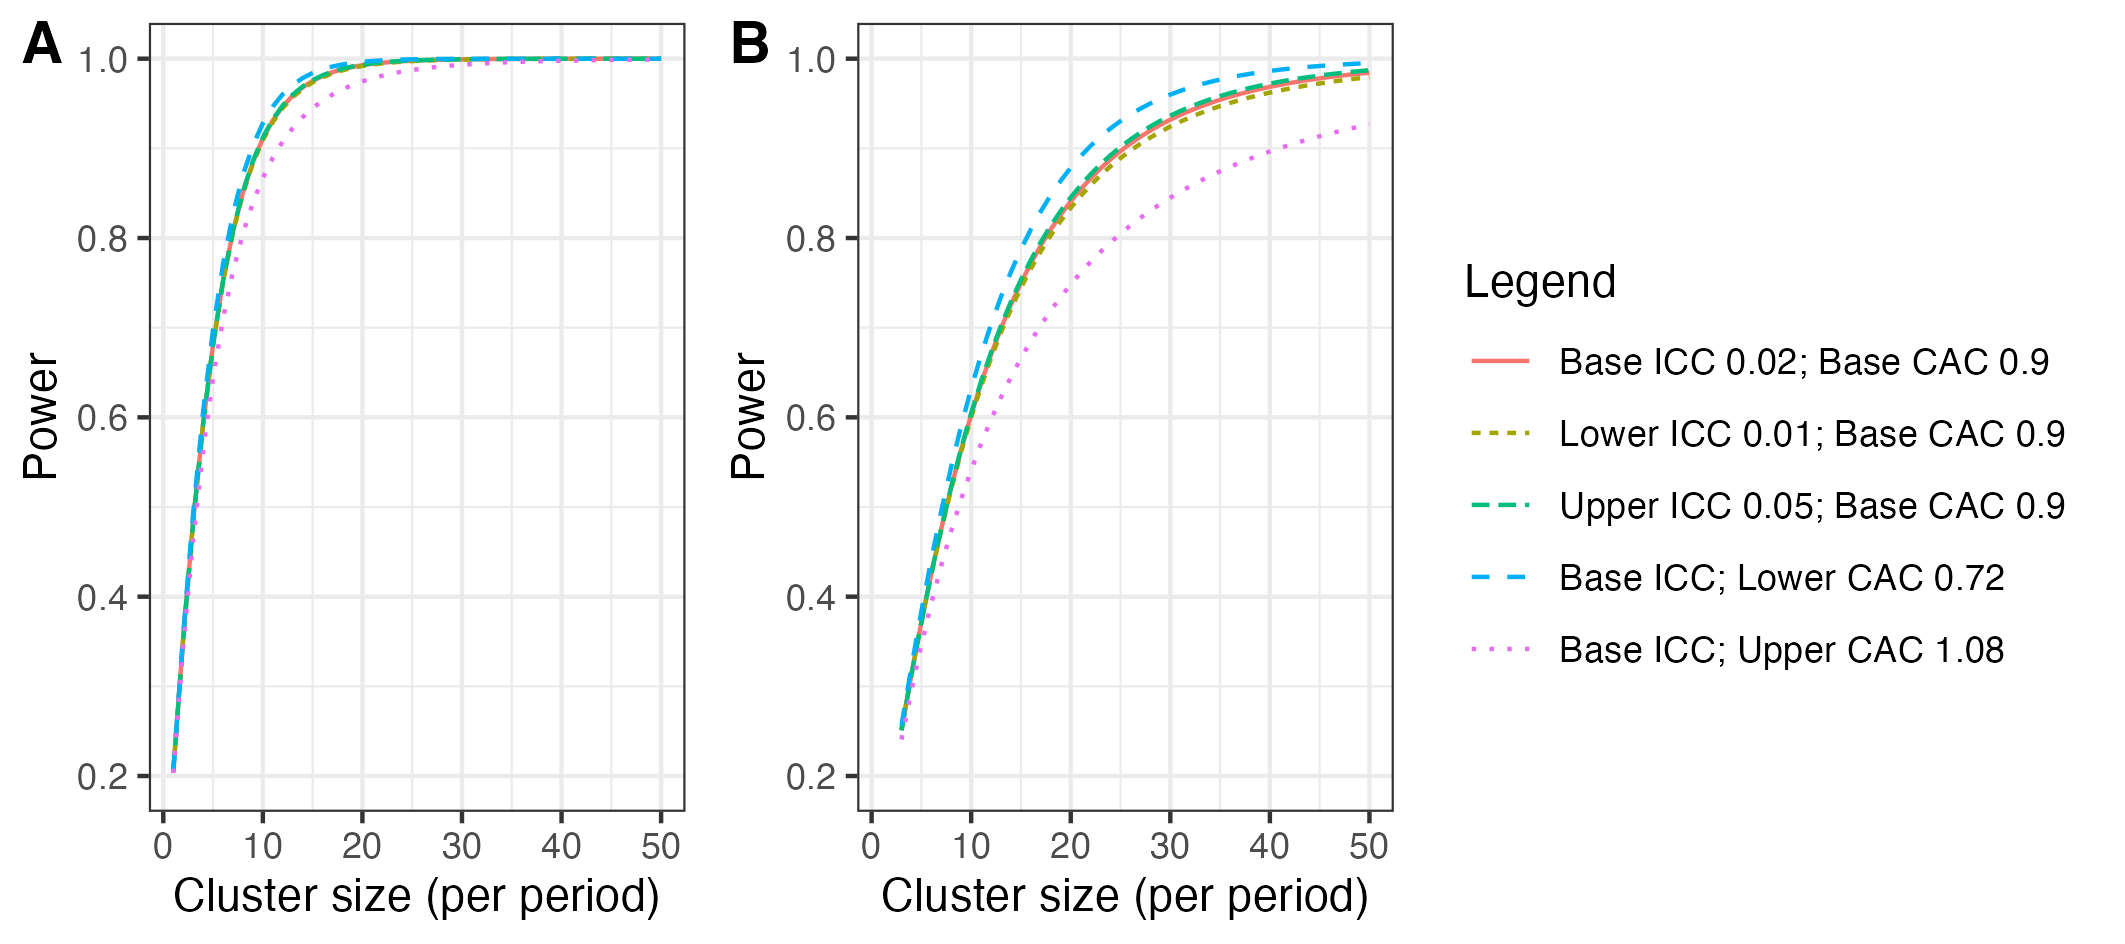
\includegraphics{./combined-power-curves.png}

}

\caption{\label{fig-power-curves}Power curves for different combinations
of cluster autocorrelations (CAC) and intra-cluster correlations (ICC).
\textbf{A)} Shows power curves assuming a reduction in the primary
outcome of in-hospital mortality within 30 days from 20\% under standard
care to 15\% after ATLS\textsuperscript{®} training. \textbf{B)} Shows
power curves assuming a reduction in the primary outcome from 10\% under
standard care to 7.5\% after ATLS\textsuperscript{®} training. Under
this scenario, we would need to increase the sample size per month to
around 30 observations to achieve 90\% powere under most combinations of
CAC and ICC.}

\end{figure}

\hypertarget{statistical-principles}{%
\subsection{Statistical principles}\label{statistical-principles}}

\hypertarget{statistical-software}{%
\subsubsection{Statistical software}\label{statistical-software}}

We will use the R Statistical Software for all
analyses\textsuperscript{7}.

\hypertarget{levels-of-statistical-significance-and-confidence}{%
\subsubsection{Levels of statistical significance and
confidence}\label{levels-of-statistical-significance-and-confidence}}

We will not perform any formal hypothesis testing as part of our planned
interim analyses. We will use a two-sided significance level of 0.05 for
all analyses, and we will report 95\% confidence intervals (CI) for all
estimates. We will not adjust for multiple testing because no secondary
outcome is regarded as singularly more important.

\hypertarget{analysis-populations}{%
\subsection{Analysis populations}\label{analysis-populations}}

The unit of randomisation is the hospital, because all units trained in
the same hospital will be treated as one cluster, but the unit of
analysis is the individual patient. The group allocation for a patient
depends on the period in which the patient was admitted to the hospital,
and patients will be considered exposed to the intervention if they were
admitted to the hospital at any time point following the transition
period. We will use an intention-to-treat approach for all analyses,
according to the planned date of transition from standard care. We might
consider a per protocol analysis if cluster deviate considerably from
the planned date of transition, using the actual date of transition as
the cut-off point. We will report the results of the per protocol
analysis as a sensitivity analysis. We will use a CONSORT diagram to
display the flow of hospitals, clusters and patients through the trial.
We will present cluster level summaries of the intervention effect. We
will report the study according to the CONSORT guidelines for
stepped-wedge randomised trials\textsuperscript{8}.

\hypertarget{baseline-analyses}{%
\subsection{Baseline analyses}\label{baseline-analyses}}

\hypertarget{cluster-characteristics}{%
\subsubsection{Cluster characteristics}\label{cluster-characteristics}}

We will describe cluster characteristics including location and size
using frequencies and percentages for discrete variables and means,
standard deviations, medians and interquartile ranges (Q1-Q3) for
continuous variables.

\hypertarget{patient-characteristics}{%
\subsubsection{Patient characteristics}\label{patient-characteristics}}

We will describe patient characteristics at baseline, meaning all
pre-training periods, per treatment group and overall using frequencies
and percentages for discrete variables and means, standard deviations,
medians and interquartile ranges (Q1-Q3) for continuous variables. We
will not adjust for clustering when presenting baseline characteristics.

\hypertarget{interim-analysis}{%
\subsection{Interim analysis}\label{interim-analysis}}

There will be one interim analyses after half of the batches have
completed the trial. The interim analyses will be assessed by the joint
Trial Steering and Data Monitoring Committee. The interim analysis will
include the baseline analyses including the frequencies and proportions
of the primary outcome in the intervention and control arms. We will
recalculate the sample size based on the observed period sizes and the
observed effect size, using the Shiny CRT Calculator\textsuperscript{4}.
In the revised sample size calculation, we will assume an ICC of 0.02,
but consider sensitivity across the range
0.01-0.05\textsuperscript{2,3}, and a CAC of 0.9, but consider
sensitivity across the range 0.8-1.0\textsuperscript{4--6}. These
assumptions are the same as in the original sample size calculation. We
will not perform any formal hypothesis testing as part of our planned
interim analyses.

\hypertarget{analysis-of-the-primary-outcome}{%
\subsection{Analysis of the primary
outcome}\label{analysis-of-the-primary-outcome}}

The primary outcomes is in-hospital mortality within 30 days of arrival
at the emergency department and will be analysed as a dichotomous
variable. We will estimate the primary intervention effect as the OR of
death between the ATLS\textsuperscript{®} and standard care arms, with
an OR \textless{} 1 indicating lower odds of death in the
ATLS\textsuperscript{®} arm compared to the standard care arm and vice
versa.

\hypertarget{main-analysis-mixed-effects-binomial-model-with-logit-link}{%
\subsubsection{Main analysis: mixed effects binomial model with logit
link}\label{main-analysis-mixed-effects-binomial-model-with-logit-link}}

We will use a mixed effects binomial model with a logit link to estimate
the OR. We will include fixed effects for period as a categorical
variable and a fixed effect for intervention exposure\footnote{\textbf{Question:}
  Should we adjust for calendar time because the last batch will be two
  years later than the first batch?}. The primary analysis will allow
for clustering as a random cluster and random cluster by period
effect\footnote{\textbf{Question:} Just a thought: keep in mind the
  complexity of the random effects structure; if it leads to convergence
  problems or overfitting, should we consider simplifying the random
  effects?}, both assumed to follow a normal distribution. The full
model is specified in Equation~\ref{eq-logit-model}. To correct the
potential inflation of the type I error rate due to small number of
clusters, the Kenward and Roger small sample correction will be used
{[}\textsuperscript{9}{]}\footnote{\textbf{Questions about Kenward and
  Roger small sample correction:} 1. What clusters do we consider here?
  Doctors? Patients? Hospitals? 2. Why use this method and not eg.
  bootstrapping? I thought Kenward and Roger was primarly used for
  linear mixed models and not for binary outcomes?}. This model will be
fitted using residual pseudo-likelihood estimation based on
linearization with subject-specific expansion (RSPL).

\begin{equation}\protect\hypertarget{eq-logit-model}{}{
\text{logit}(\text{Pr}(Y_{bkti} = 1)) = \mu + \beta_{bt} + \theta X_{bkt} + \alpha_{bk} + \gamma_{bkt} 
}\label{eq-logit-model}\end{equation}

Where:

\begin{itemize}
\tightlist
\item
  \(\text{Pr}(Y_{bkti} = 1)\): the probability of death for patient
  \(i = 1, \dotsc,m\) in cluster \(k = 1, \dotsc, 30\) during period
  \(t = 1, \dotsc, 12\) in batch \(b = 1, \dotsc, 6\).
\item
  \(\mu\): the intercept, representing the baseline log-odds of the
  outcome when all predictors are set to 1.
\item
  \(\beta_{bt}\): the fixed effect of period \(t\) in batch \(b\),
  accounting for a separate period effect for each batch, so that there
  is a total of 72 period effects.\footnote{\textbf{Question:} The model
    will estimate some 78 parameters. Is this a problem considering the
    low number of participants per period?}
\item
  \(\theta\): the fixed effect of intervention exposure, representing
  the effect of ATLS® exposure on the probability of death.
\item
  \(X_{bkt}\): the treatment arm indicator for patient \(i\) in cluster
  \(k\) during period \(t\) in batch \(b\), with \(X_{bkt} = 1\) for
  ATLS\textsuperscript{®} and \(X_{bkt} = 0\) for standard care.
\item
  \(\alpha_{bk}\): the random effect of cluster \(k\) in batch \(b\),
  representing the variability in outcomes between different clusters
  (hospitals) across batches.
\item
  \(\gamma_{bkt}\): the random effect of cluster \(k\) in period \(t\)
  in batch \(b\), accounting for the random variation within clusters
  across periods and batches, including potential interaction effects
  between clusters and time.
\end{itemize}

We will present the effect of ATLS\textsuperscript{®} exposure as an
odds ratio (OR) for mortality with an associated 95\% CI, using the
standard care arm as the reference. Additionally, we will present the
risk difference with a 95\% CI. The randomization within each batch will
be balanced based on cluster size, defined as the expected monthly
volume of eligible patient participants. Therefore, no further
adjustment for cluster size will be made in the main analysis.

\hypertarget{sensitivity-analyses}{%
\subsubsection{Sensitivity analyses}\label{sensitivity-analyses}}

The sensitivity analyses will be conducted to assess the robustness of
the main analysis results to different model specifications. We will
first model the primary outcome using an identity link function to
estimate the risk difference instead of the OR. Henceforth, each
additional sensitivity analyses will be operationalised using two
separate models, one with the logit link and one with the identity link.
We will first explore more complex correlation structures. We will then
model time using a spline function. Finally, we will conduct a fully
adjusted covariate analysis.

\hypertarget{model-with-identify-link}{%
\paragraph{Model with identify link}\label{model-with-identify-link}}

We will use an identity link used to estimate the risk difference,
meaning that the coefficient will be interpreted as the difference in
the probability of death between the ATLS\textsuperscript{®} and
standard care arms. We will present the risk difference with a 95\% CI.
This model is specified in Equation~\ref{eq-identity-model} and will
also be fitted using RSPL. If the binomial model with the identity link
does not converge then only a odds ratio will be reported.

\begin{equation}\protect\hypertarget{eq-identity-model}{}{
\text{Pr}(Y_{bkti} = 1) = \mu + \beta_{bt} + \theta X_{bkt} + \alpha_{bk} + \gamma_{bkt} 
}\label{eq-identity-model}\end{equation}

Where:

\begin{itemize}
\tightlist
\item
  \(\mu\): the intercept, representing the baseline probability of the
  outcome when all predictors are zero.
\end{itemize}

\hypertarget{models-with-different-correlation-structure}{%
\paragraph{Models with different correlation
structure}\label{models-with-different-correlation-structure}}

We will explore if models with more complicated correlation structures
are a better fit to the data. These models are not being used as our
primary analysis models as there is limited understanding as to when
such models will converge and how to choose between the various
different correlation structures which might be plausible. First, we
will include a discrete time decay correlation structure including a
random cluster effect with auto-regressive structure (AR(1)), described
in Equation~\ref{eq-ar1}.

\begin{equation}\protect\hypertarget{eq-ar1}{}{
\alpha_{bk, t} = \rho \alpha_{bk, t-1} + \epsilon_{t}, \quad \epsilon_{t} \sim N(0, \sigma^2_\alpha)
}\label{eq-ar1}\end{equation}

Where:

\begin{itemize}
\tightlist
\item
  \(\rho\): the correlation between the random effects of two
  consecutive periods, the period \(t\) and the period \(t-1\),
  reflecting how outcomes in one period are correlated with outcomes in
  the previous period within the same cluster.
\item
  \(\alpha_{bk, t}\): the random effect of cluster \(k\) in period \(t\)
  in batch \(b\). This represents the variation in the outcome that is
  specific to each cluster and period, accounting for time-related
  effects.
\item
  \(\epsilon_{t}\) is the error term for period \(t\), which is assumed
  to be normally distributed with mean 0 and variance
  \(\sigma^2_\alpha\).
\end{itemize}

To allow for the randomisation by batches, we will also include a
different secular trend for each batch as a random effect interaction
term between batch and period. The full model is specified in
Equation~\ref{eq-logit-ar1}.

\begin{equation}\protect\hypertarget{eq-logit-ar1}{}{
g(\text{Pr}(Y_{bkti} = 1)) = \mu + \beta_{bt} + \theta X_{bkt} + \alpha_{bk,t} + \gamma_{bkt} + \delta_{bt}
}\label{eq-logit-ar1}\end{equation}

Where:

\begin{itemize}
\tightlist
\item
  \(g(\cdot)\): the link function.
\item
  \(\alpha_{bk,t}\): the updated random effect of cluster \(k\) in batch
  \(b\) during period \(t\) with the AR(1) correlation structure. This
  accounts for correlation between adjacent periods in the same cluster.
\item
  \(\delta_{bt}\): the random effect of batch \(b\) during period \(t\),
  which captures any variability across different batches over time.
\end{itemize}

\hypertarget{models-with-random-cluster-by-intervention-effects}{%
\paragraph{Models with random cluster by intervention
effects}\label{models-with-random-cluster-by-intervention-effects}}

Models will also be extended to include random cluster by intervention
effects (with a non-zero covariance term) to examine if results are
sensitive to the assumption of no intervention by cluster interaction.
The model is specified in
Equation~\ref{eq-logit-random-cluster-intervention}.

\begin{equation}\protect\hypertarget{eq-logit-random-cluster-intervention}{}{
g(\text{Pr}(Y_{bkti} = 1)) = \mu + \beta_{bt} + \theta X_{bkt} + \alpha_{bk} + \gamma_{bkt} + u_{bk} \times X_{bkt}
}\label{eq-logit-random-cluster-intervention}\end{equation}

Where:

\begin{itemize}
\tightlist
\item
  \(u_{bk}\): the random effect of cluster \(k\) by intervention
  interaction.
\item
  \(X_{bkt}\): the treatment arm indicator for patient \(i\) in cluster
  \(k\) during period \(t\).
\item
  \$u\_\{bk\} \textbackslash times X\_\{bkt\} \$: the random interaction
  effect between the intervention and cluster \(k\).
\end{itemize}

\hypertarget{models-with-time-modelled-with-a-spline-function}{%
\paragraph{Models with time modelled with a spline
function}\label{models-with-time-modelled-with-a-spline-function}}

We will further explore the potential for a time-varying treatment
effect\textsuperscript{10}. To explore if the fixed period effect is
both parsimonious and adequate to represent the extent of any underlying
secular trend, we will model the time effect using natural cubic splines
with knots at the equally spaced time points 3, 6 and 9. This will
result in five spline basis functions, because the natural cubic splines
are modelled with three degrees of freedom but are constrained to be
linear before the first and after the last knot. The model is specified
in Equation~\ref{eq-spline-model}.

\begin{equation}\protect\hypertarget{eq-spline-model}{}{
g(\text{Pr}(Y_{bkti} = 1)) = \mu + \sum_{j=1}^5 \beta_j S_j(t, \{3, 6, 9\}) + \theta X_{bkt} + \alpha_{bk} + \gamma_{bkt}
}\label{eq-spline-model}\end{equation}

Where:

\begin{itemize}
\tightlist
\item
  \(S_j(t, \{3, 6, 9\})\): the natural cubic spline basis functions with
  knots placed at times 3, 6 and 9.
\item
  \(\beta_j\): the coefficient for the \(j\)-th spline basis function.
\end{itemize}

\hypertarget{models-exploring-lag-and-weaning-effects}{%
\paragraph{Models exploring lag and weaning
effects}\label{models-exploring-lag-and-weaning-effects}}

Models will also be extended to include an interaction between treatment
and number of periods since first treated, to examine if there is any
indication of a relationship between duration of exposure to the
intervention and outcomes. This will allow us to model different lag
effects (whereby it takes time for the intervention to become embedded
within the culture before its impact can properly start to be realised);
as well as weaning effects (whereby the effect of the intervention
starts to decrease -- or fade). This type of analysis attempts to
disentangle how some clusters end up having a long exposure to the
intervention and others have a much shorter exposure time. The model is
specified in Equation~\ref{eq-lag-weaning-model}.

\begin{equation}\protect\hypertarget{eq-lag-weaning-model}{}{
g(\text{Pr}(Y_{bkti} = 1)) = \mu + \beta_{bt} + \theta X_{bkt} + \theta_{\text{int}} X_{bkt} \times T_{bkt} + \alpha_{bk} + \gamma_{bkt}
}\label{eq-lag-weaning-model}\end{equation}

Where:

\begin{itemize}
\tightlist
\item
  \(\theta_{\text{int}}\) is the coefficient for the interaction between
  treatment and time since first treated.
\item
  \(T_{bkt}\) is the number of periods since first treated.
\end{itemize}

\hypertarget{adjusted-analyses}{%
\subsubsection{Adjusted analyses}\label{adjusted-analyses}}

Fully adjusted covariate analysis will additionally adjust
for\footnote{\textbf{Questions:} 1. Should we adjust for calendar time
  because the last batch will be two years later than the first batch?
  2. Should we add it as covariate in the list above? 3. Should it be
  continuous (e.g., months since the study started) or categorical
  calendar time (if you expect non-linear trends or stepwise changes
  over years)? 4. Should we analyse Time Since Admission? Depending on
  the nature of the trauma, the time since patient admission might also
  influence outcomes, especially if the timing of interventions or care
  decisions plays a critical role. Eg. time from admission to surgery.}
(expected \% missing data in parentheses):

\begin{itemize}
\tightlist
\item
  Age (\textless5\%)
\item
  Sex (\textless5\%)
\item
  Systolic blood pressure (25\%)
\item
  Glasgow Coma Scale (25\%)
\item
  Injury Severity Score (10\%)
\item
  Mechanism of injury (10\%)
\end{itemize}

These are known individual-level prognostic factors for the primary
outcome. These covariates will be included in the models specified in
Equation~\ref{eq-logit-model} and Equation~\ref{eq-identity-model} as
fixed effects. We will model the continuous covariates assuming linear
effects.

\hypertarget{subgroup-analyses}{%
\subsubsection{Subgroup analyses}\label{subgroup-analyses}}

We will perform the following subgroup analyses\footnote{\textbf{Question:}
  Are we exploring too many subgroups?}:

\begin{itemize}
\tightlist
\item
  geographical region, defined using the state in which the
  participating hospital is located. Demonstrating the consistency of
  any effect across multiple regions will enhance the generalisibility
  of the results;
\item
  age groups, defined as older adolescents (15-19 years), young adults
  (20-24 years), adults (25-59 years), and older adults (60 years and
  older) {[}\textsuperscript{11};
\item
  sex, using the levels male and female;
\item
  clinical cohorts, defined as blunt multisystem trauma, penetrating
  trauma, and severe isolated traumatic brain injury, with modification
  to avoid overlap between the cohorts; and
\item
  cluster size (number of patients per hospital)
\end{itemize}

These subgroup analyses will be conducted by adding the subgroup
variable and the interaction between the subgroup variable and the
intervention exposure variable as fixed effects to the models specified
in Equation~\ref{eq-logit-model} and Equation~\ref{eq-identity-model}.

\hypertarget{treatment-of-missing-data}{%
\subsubsection{Treatment of missing
data}\label{treatment-of-missing-data}}

We will present the frequency and percentage of missing data for all
variables. If the percentage of missing data for the primary outcome is
less than 10\%, we will perform a complete case analysis. If the
percentage of missing data for the primary outcome is 10\% or more, we
will handle missing data depending on the missing data mechanism. If the
data are missing at random (MAR), we will perform multiple imputation
using multiple imputation by chained equations (MICE), imputing data for
the primary outcome as well as all covariates included in the fully
adjusted model. The number of imputations will be determined by the
percentage of missing data, with a minimum of 20 imputations. If there
is evidence that the data are missing not at random (MNAR), we will
explore the impact of this assumption using a sensitivity analysis
(e.g., pattern mixture models or selection models) to assess how robust
our findings are to different assumptions about the missing data
mechanism. Additionally, we will perform diagnostic checks after
multiple imputation to ensure the quality of the imputation process,
including comparing distributions of observed and imputed data and
checking convergence.

\hypertarget{analysis-of-secondary-outcomes}{%
\subsection{Analysis of secondary
outcomes}\label{analysis-of-secondary-outcomes}}

\hypertarget{all-cause-mortality-within-24-hours-30-days-and-three-months-of-arrival-at-the-emergency-department}{%
\subsubsection{All cause mortality within 24 hours, 30 days and three
months of arrival at the emergency
department}\label{all-cause-mortality-within-24-hours-30-days-and-three-months-of-arrival-at-the-emergency-department}}

We will use the model with the logit link specified in
Equation~\ref{eq-logit-model} and the model with the identity link
specified in Equation~\ref{eq-identity-model} to estimate the OR and
risk difference for these mortality outcomes.

\hypertarget{quality-of-life-within-seven-days-of-discharge-and-at-30-days-and-three-months-of-arrival-at-the-emergency-department}{%
\subsubsection{Quality of life within seven days of discharge, and at 30
days and three months of arrival at the emergency
department}\label{quality-of-life-within-seven-days-of-discharge-and-at-30-days-and-three-months-of-arrival-at-the-emergency-department}}

Quality of life will be measured by the official and validated
translations of the EQ5D5L. This tool assesses five dimensions of
health-related quality of life: mobility, self-care, usual activities,
pain/discomfort, and anxiety/depression. Each dimension is rated on a
likert scale from 1 to 5. There is also a visual analogue scale (VAS)
for self-rated quality of life, ranging from 0 to 100. For each of the
five dimensions we will use a mixed effects ordinal model as specified
in Equation~\ref{eq-ordinal-model}.

\begin{equation}\protect\hypertarget{eq-ordinal-model}{}{
\text{logit}(\text{Pr}(Y_{bkti} \leq j)) = \mu_j + \beta_{bt} + \theta X_{bkt} + \alpha_{bk} + \gamma_{bkt}
}\label{eq-ordinal-model}\end{equation}

Where:

\begin{itemize}
\tightlist
\item
  \(\mu_j\): the intercept for the \(j\)-th category of the EQ5D
  dimension (\(j\) = 1, 2, 3, 4, 5).
\end{itemize}

The VAS will be analysed using a linear mixed effects model as specified
in Equation~\ref{eq-linear-model}.

\begin{equation}\protect\hypertarget{eq-linear-model}{}{
\text{VAS}_{bkti} = \mu + \beta_{bt} + \theta X_{bkt} + \alpha_{bk} + \gamma_{bkt} + \epsilon_{bkti}, \quad \epsilon_{bkti} \sim N(0, \sigma^2)
}\label{eq-linear-model}\end{equation}

Where:

\begin{itemize}
\tightlist
\item
  \(\epsilon_{bkti}\): the error term for patient \(i\) in cluster \(k\)
  in period \(t\) in batch \(b\), assumed to be normally distributed
  with mean 0 and variance \(\sigma^2\).
\end{itemize}

\hypertarget{disability-within-seven-days-of-discharge-and-at-30-days-and-three-months-of-arrival-at-the-emergency-department}{%
\subsubsection{Disability within seven days of discharge, and at 30 days
and three months of arrival at the emergency
department}\label{disability-within-seven-days-of-discharge-and-at-30-days-and-three-months-of-arrival-at-the-emergency-department}}

We will measure disability using the WHO Disability Assessment Schedule
2.0 (WHODAS 2.0)\textsuperscript{12}. This tool assesses six domains of
functioning: cognition, mobility, self-care, getting along, life
activities, and participation. Each domain is rated on a likert scale
from 1 to 5, with 1 indicating no difficulties and 5 indicating extreme
difficulties. We will analyse each domain separately using a mixed
effects ordinal model as specified in Equation~\ref{eq-ordinal-model}.
We will also calculate a WHODAS 2.0 summary score using the method
referred to as the ``complex scoring'' method. This method involves
summing the item scores within each of the six domains, then summing the
scores of all domains, and finally transforming the total score to a
0-100 scale. We will analyse the summary score using a linear mixed
effects model as specified in Equation~\ref{eq-linear-model}.

\hypertarget{return-to-work-at-30-days-and-three-months-after-arrival-at-the-emergency-department}{%
\subsubsection{Return to work at 30 days and three months after arrival
at the emergency
department}\label{return-to-work-at-30-days-and-three-months-after-arrival-at-the-emergency-department}}

We will analyse return to work as a dichotomous variable using a mixed
effects binomial model with a logit link as specified in
Equation~\ref{eq-logit-model}.

\hypertarget{length-of-emergency-department-stay}{%
\subsubsection{Length of emergency department
stay}\label{length-of-emergency-department-stay}}

We will analyse length of emergency department stay as a continuous
variable using a linear mixed effects model as specified in
Equation~\ref{eq-linear-model}.

\hypertarget{length-of-hospital-stay}{%
\subsubsection{Length of hospital stay}\label{length-of-hospital-stay}}

We will analyse length of hospital stay as a continuous variable using a
linear mixed effects model as specified in
Equation~\ref{eq-linear-model}.

\hypertarget{intensive-care-unit-admission}{%
\subsubsection{Intensive care unit
admission}\label{intensive-care-unit-admission}}

We will analyse intensive care unit admission as a dichotomous variable
using a mixed effects binomial model with a logit link as specified in
Equation~\ref{eq-logit-model}.

\hypertarget{length-of-intensive-care-unit-stay}{%
\subsubsection{Length of intensive care unit
stay}\label{length-of-intensive-care-unit-stay}}

We will analyse length of intensive care unit stay as a continuous
variable using a linear mixed effects model as specified in
Equation~\ref{eq-linear-model}.

\hypertarget{adherence-to-atls-principles-during-initial-patient-resuscitation}{%
\subsubsection{\texorpdfstring{Adherence to ATLS\textsuperscript{®}
principles during initial patient
resuscitation}{Adherence to ATLS® principles during initial patient resuscitation}}\label{adherence-to-atls-principles-during-initial-patient-resuscitation}}

We will assess adherence to ATLS® principles using a 14-item checklist
that covers the key steps of the ATLS® primary survey. Adherence will be
measured as the proportion of steps completed, with 100\% adherence
defined as completing all 14 steps. We will analyse adherence using a
mixed-effects beta regression model with a logit link as specified in
Equation~\ref{eq-beta-model}.

\begin{equation}\protect\hypertarget{eq-beta-model}{}{
\text{logit}(\text{E}(Y_{bkti})) = \mu + \beta_{bt} + \theta X_{bkt} + \alpha_{bk} + \gamma_{bkt}
}\label{eq-beta-model}\end{equation}

Where:

\begin{itemize}
\tightlist
\item
  \(\text{E}(Y_{bkti})\): The expected proportion of completed ATLS
  steps for patient \(i\) in cluster \(k\) during period \(t\) in batch
  \(b\).
\item
  \(\mu\): The intercept, representing the baseline log-odds of
  completing ATLS steps when all predictors are set to 1.
\item
  \(\beta_{bt}\): The fixed effect of period \(t\) in batch \(b\),
  allowing for different period effects for each batch.
\item
  \(\theta\): The fixed effect of ATLS exposure, representing the effect
  of the intervention on adherence to ATLS principles.
\item
  \(X_{bkt}\): The treatment arm indicator for patient \(i\) in cluster
  \(k\) during period \(t\) in batch \(b\) (1 for ATLS, 0 for standard
  care).
\item
  \(\alpha_{bk}\): The random effect of cluster \(k\) in batch \(b\),
  capturing variability in adherence across clusters (hospitals).
\item
  \(\gamma_{bkt}\): The random effect of cluster \(k\) in period \(t\)
  within batch \(b\), accounting for within-cluster variability across
  time periods and batches.
\end{itemize}

\hypertarget{references}{%
\section*{References}\label{references}}
\addcontentsline{toc}{section}{References}

\hypertarget{refs}{}
\begin{CSLReferences}{0}{0}
\leavevmode\vadjust pre{\hypertarget{ref-Kasza2022}{}}%
\CSLLeftMargin{1. }%
\CSLRightInline{Kasza, J. \emph{et al.} The batched stepped wedge
design: A design robust to delays in cluster recruitment. \emph{Stat
Med} \textbf{41}, 3627--3641 (2022).}

\leavevmode\vadjust pre{\hypertarget{ref-Campbell2005}{}}%
\CSLLeftMargin{2. }%
\CSLRightInline{Campbell, M. K. \emph{et al.} Determinants of the
intracluster correlation coefficient in cluster randomized trials: The
case of implementation research. \emph{Clinical Trials} \textbf{2},
99--107 (2005).}

\leavevmode\vadjust pre{\hypertarget{ref-Eldridge2015}{}}%
\CSLLeftMargin{3. }%
\CSLRightInline{Eldridge, S. M. \emph{et al.} How big should the pilot
study for my cluster randomised trial be? \emph{Stat Methods Med Res}
\textbf{25}, 1039--1056 (2015).}

\leavevmode\vadjust pre{\hypertarget{ref-Hemming2020Feb}{}}%
\CSLLeftMargin{4. }%
\CSLRightInline{Hemming, K. \emph{et al.} A tutorial on sample size
calculation for multiple-period cluster randomized parallel, cross-over
and stepped-wedge trials using the shiny CRT calculator. \emph{Int J
Epidemiol} \textbf{49}, 979--995 (2020).}

\leavevmode\vadjust pre{\hypertarget{ref-Martin2016}{}}%
\CSLLeftMargin{5. }%
\CSLRightInline{Martin, J. \emph{et al.} Intra-cluster and inter-period
correlation coefficients for cross-sectional cluster randomised
controlled trials for type-2 diabetes in UK primary care. \emph{Trials}
\textbf{17}, (2016).}

\leavevmode\vadjust pre{\hypertarget{ref-Korevaar2021}{}}%
\CSLLeftMargin{6. }%
\CSLRightInline{Korevaar, E. \emph{et al.} Intra-cluster correlations
from the CLustered OUtcome dataset bank to inform the design of
longitudinal cluster trials. \emph{Clinical Trials} \textbf{18},
529--540 (2021).}

\leavevmode\vadjust pre{\hypertarget{ref-R}{}}%
\CSLLeftMargin{7. }%
\CSLRightInline{R Core Team. \emph{R: A language and environment for
statistical computing}. (R Foundation for Statistical Computing, 2023).}

\leavevmode\vadjust pre{\hypertarget{ref-Hemming2018}{}}%
\CSLLeftMargin{8. }%
\CSLRightInline{Hemming, K. \emph{et al.} Reporting of stepped wedge
cluster randomised trials: Extension of the CONSORT 2010 statement with
explanation and elaboration. \emph{BMJ} k1614 (2018).}

\leavevmode\vadjust pre{\hypertarget{ref-kenward_small_1997}{}}%
\CSLLeftMargin{9. }%
\CSLRightInline{Kenward, M. G. \emph{et al.} Small {Sample} {Inference}
for {Fixed} {Effects} from {Restricted} {Maximum} {Likelihood}.
\emph{Biometrics} \textbf{53}, 983--997 (1997).}

\leavevmode\vadjust pre{\hypertarget{ref-kenny_analysis_2022}{}}%
\CSLLeftMargin{10. }%
\CSLRightInline{Kenny, A. \emph{et al.} Analysis of stepped wedge
cluster randomized trials in the presence of a time-varying treatment
effect. \emph{Statistics in medicine} 10.1002/sim.9511 (2022).}

\leavevmode\vadjust pre{\hypertarget{ref-Diaz2021}{}}%
\CSLLeftMargin{11. }%
\CSLRightInline{Diaz, T. \emph{et al.} A call for standardised
age-disaggregated health data. \emph{The Lancet Healthy Longevity}
\textbf{2}, e436--e443 (2021).}

\leavevmode\vadjust pre{\hypertarget{ref-ustun_measuring_2010}{}}%
\CSLLeftMargin{12. }%
\CSLRightInline{Ustun, T. B. \emph{et al.} \emph{Measuring {Health} and
{Disability}: {Manual} for {WHO} {Disability} {Assessment} {Schedule}
({WHODAS} 2.0)}. (World Health Organization, 2010).}

\end{CSLReferences}



\end{document}
